\subsection{Rapid Test Statistics}
\label{subsec:results_rapid_test_statistics}

An important feature in our model is that our rapid tests are imperfectly specific and
imperfectly sensitive. Especially when people have not become infectious yet they are
likely to return a false positive result. Here we look at how rapid tests expanded over
time and to what degree they are useful as a screening device despite missing positive
cases and returning false positive results.

We start with the share of the population doing a rapid test, receiving a positive rapid
test and receiving a negative rapid test over time by the channel through which the test
was demanded in Figures~\ref{fig:rapid_test_demand_by_channel,
fig:pos_rapid_tests_by_channel} and \ref{fig:neg_rapid_tests_by_channel} respectively.
Overall, the share of the population getting a rapid test on a given day increases from
2\% in Mid March to over 10\% by May. The work rapid tests are a little ragged because of
public holidays and weekend effects that lead to jumps around Mondays. For education
rapid tests both vacations (first half of April) as well as the opening of schools in May
are very visible in the rapid test demand. Overall, work tests make up the largest
fraction of rapid tests. The image is very similar for the share of positive tests,
except that the overall number of positive tests starts decreasing in May as rapid test
expansion comes to a halt and cases fall, especially the positive share of private rapid
tests falls as less and less individuals seek a rapid test because of a positive test in
their household.

\begin{figure}[ht] % Share tested per day
  \centering
  \begin{subfigure}[b]{0.3\textwidth}
      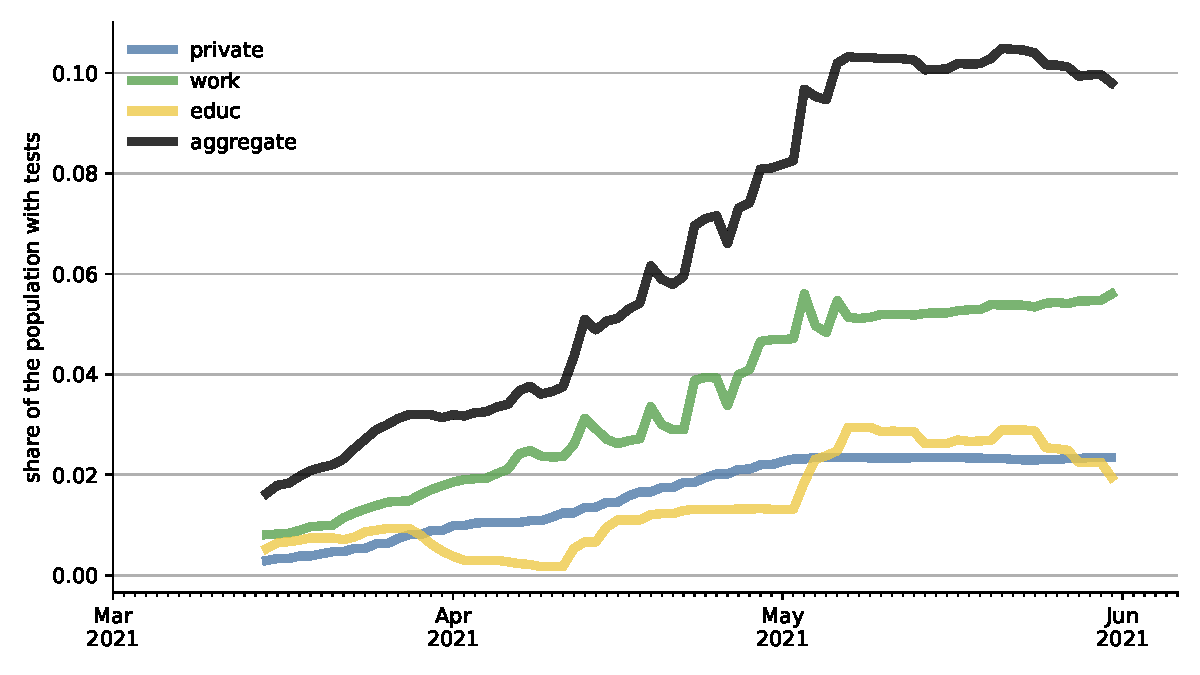
\includegraphics[width=\textwidth]{figures/results/figures/rapid_test_statistics/popshare_tested}
      \caption{Share of the Population Doing a Rapid Test Because of Different Channels
      on a Given Day}
      \label{fig:rapid_test_demand_by_channel}
  \end{subfigure}
  \hfill
  \begin{subfigure}[b]{0.3\textwidth}
      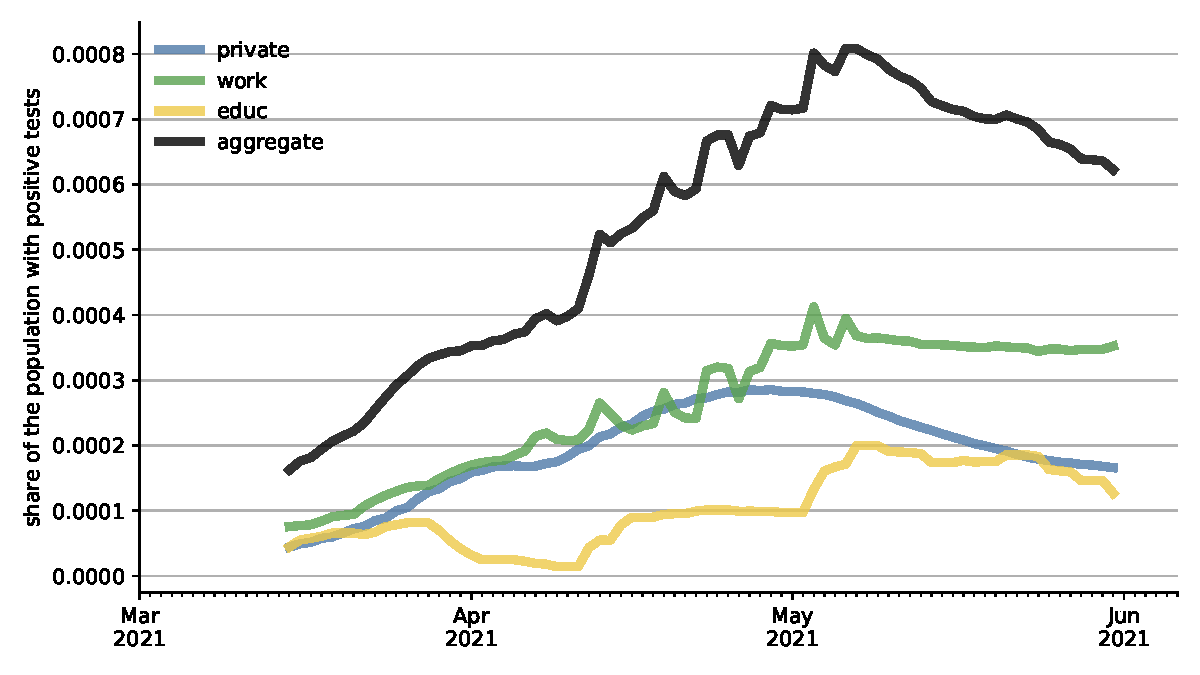
\includegraphics[width=\textwidth]{figures/results/figures/rapid_test_statistics/popshare_tested_positive}
      \caption{Share of the Population Testing Positive Because of Different Channels
      on a Given Day}
      \label{fig:pos_rapid_tests_by_channel}
  \end{subfigure}
  \hfill
  \begin{subfigure}[b]{0.3\textwidth}
      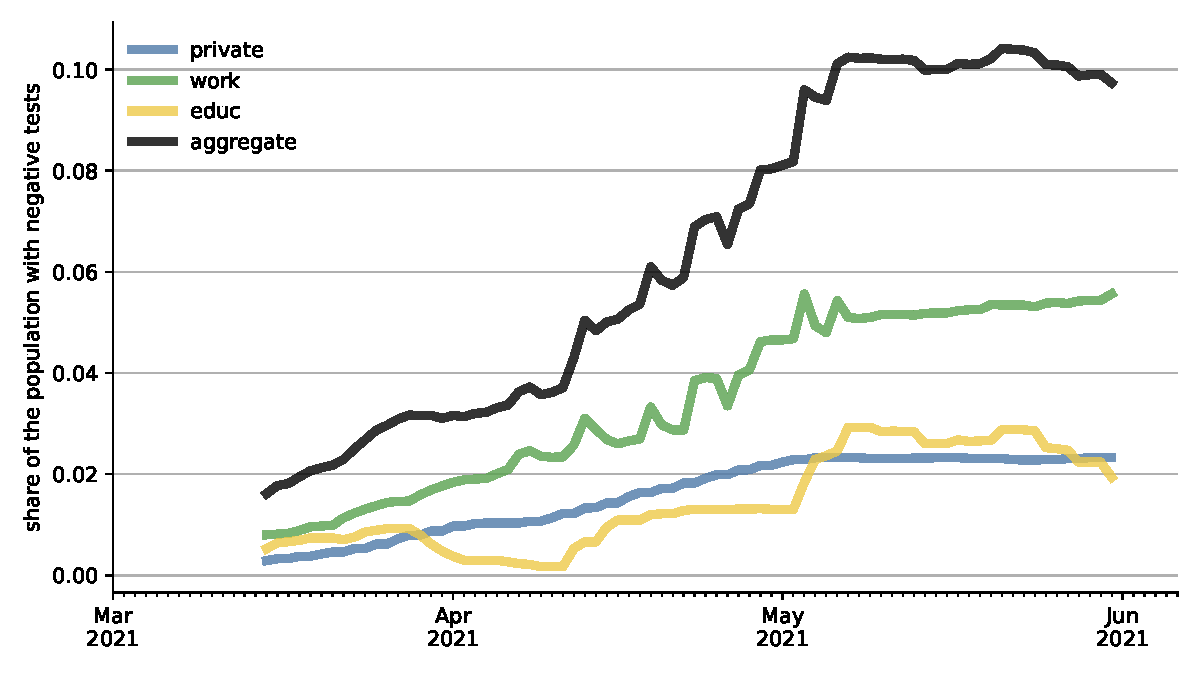
\includegraphics[width=\textwidth]{figures/results/figures/rapid_test_statistics/popshare_tested_negative}
      \caption{Share of the Population Testing Negative Because of Different Channels
      on a Given Day}
      \label{fig:neg_rapid_tests_by_channel}
  \end{subfigure}
  \caption{Rapid Test Shares in the Population by Channel}
  \floatfoot{\noindent \textit{Note:}
    Rapid tests in the education setting are demanded by teachers (nursery, preschool and
    school) as well as school pupils. After Easter the required frequency of tests is
    increased from once per week to twice per week. Work rapid tests are demanded by
    individuals that still have work contacts, i.e. do not work from home. The share of
    employers offering rapid tests increases over the time frame and the frequency of
    testing is also increased. Tests are demanded by individuals for one of three private
    reasons: having developed symptoms without access to a PCR test, having a household
    member that has tested positive or developed symptoms or having planned weekly
    meeting with friends. The left figure shows the share of the population demanding a
    rapid test on a given day. The middle figure shows the share of the population
    testing positive on a given day (true and false positives). The right figure shows
    the share of the population testing negative on a given day (true and false
    negatives).}
\end{figure}


\begin{figure}   % Number of True Positive / False Positive / True Negative / False Negative
    \centering
    \begin{subfigure}[b]{0.425\textwidth}
        \centering
        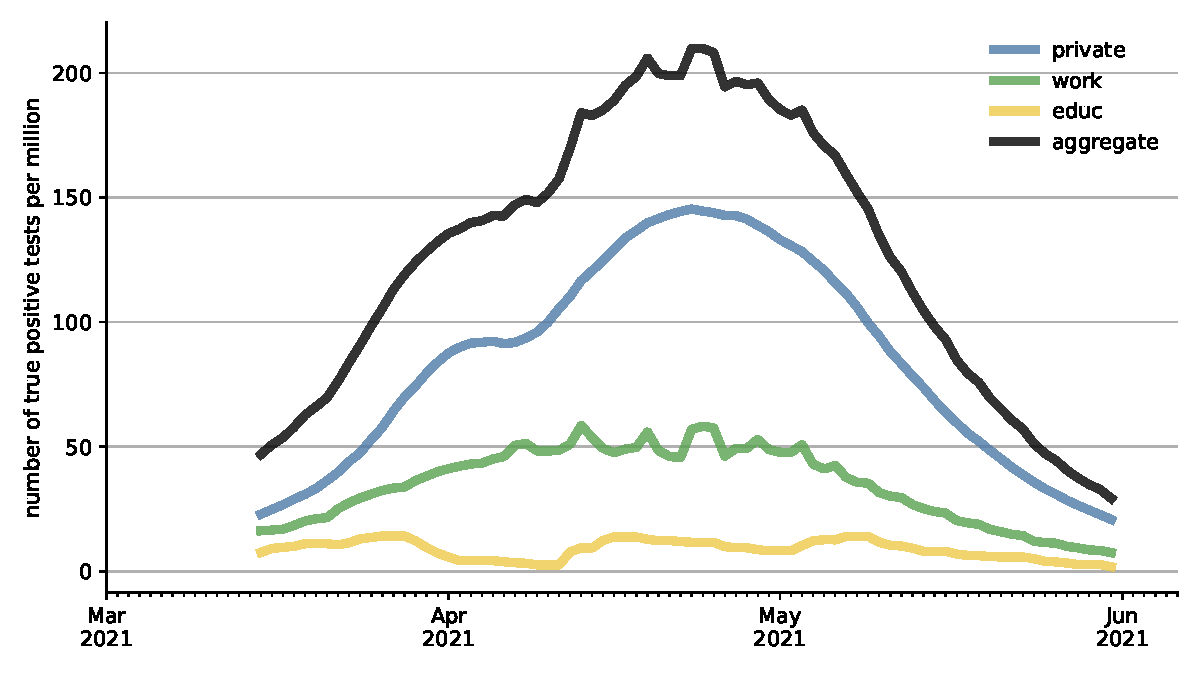
\includegraphics[width=\textwidth]{figures/results/figures/rapid_test_statistics/number_true_positive}
        \caption{Number of Discovered Cases Due to Rapid Tests by Channel}
        \label{fig:rapid_tests_number_true_positive}
    \end{subfigure}
    \hfill
    \begin{subfigure}[b]{0.425\textwidth}
        \centering
        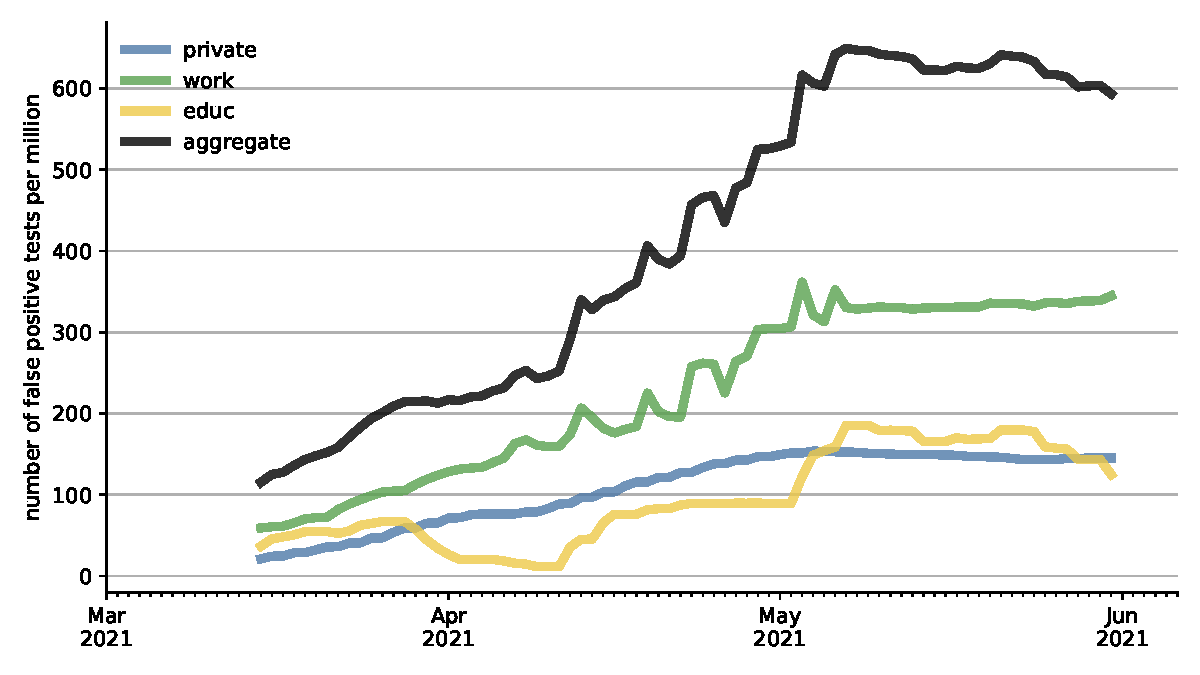
\includegraphics[width=\textwidth]{figures/results/figures/rapid_test_statistics/number_false_positive}
        \caption{Number of False Positive Rapid Tests by Channel}
        \label{fig:rapid_tests_number_false_positive}
    \end{subfigure}
    \vskip3ex
    \begin{subfigure}[b]{0.425\textwidth}
        \centering
        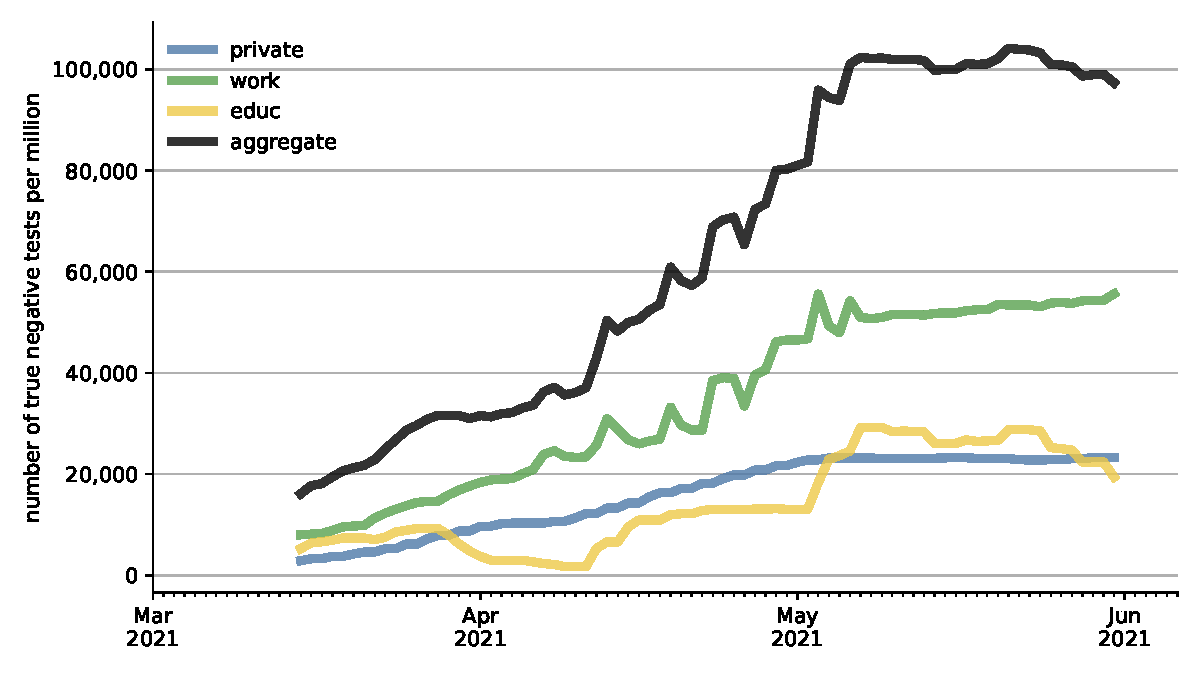
\includegraphics[width=\textwidth]{figures/results/figures/rapid_test_statistics/number_true_negative}
        \caption{Number of True Negative Rapid Tests by Channel}
        \label{fig:rapid_tests_number_true_negative}
    \end{subfigure}
    \hfill
    \begin{subfigure}[b]{0.425\textwidth}
        \centering
        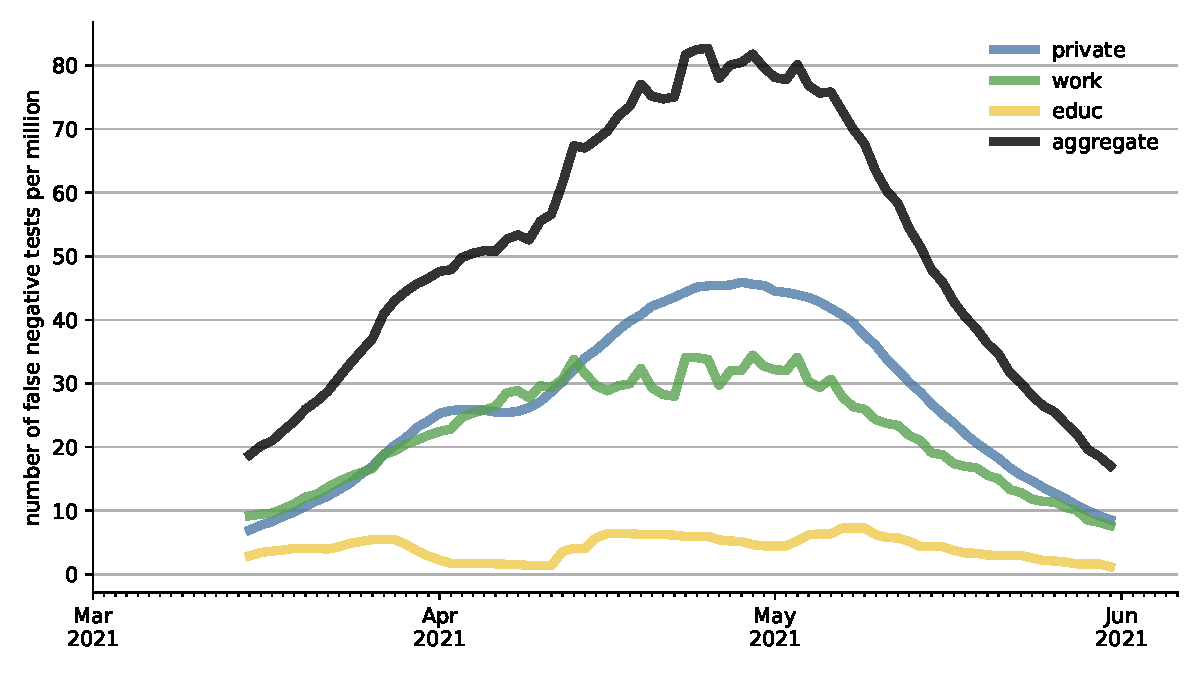
\includegraphics[width=\textwidth]{figures/results/figures/rapid_test_statistics/number_false_negative}
        \caption{Number of False Negative Rapid Tests by Channel}
        \label{fig:rapid_tests_number_false_negative}
    \end{subfigure}
    \vskip3ex
    \caption{Rapid Test Results}
    \label{fig:rapid_test_results_numbers}

    \floatfoot{\noindent \textit{Note:}
      The number of rapid tests of each category are upscaled to the full German
      population. \textcolor{red}{To be written.}
    }
\end{figure}


\begin{figure} % True Positive / False Positive / True Negative / False Negative Rate
    \centering
    % \begin{subfigure}[b]{0.425\textwidth}
    %     \centering
    %     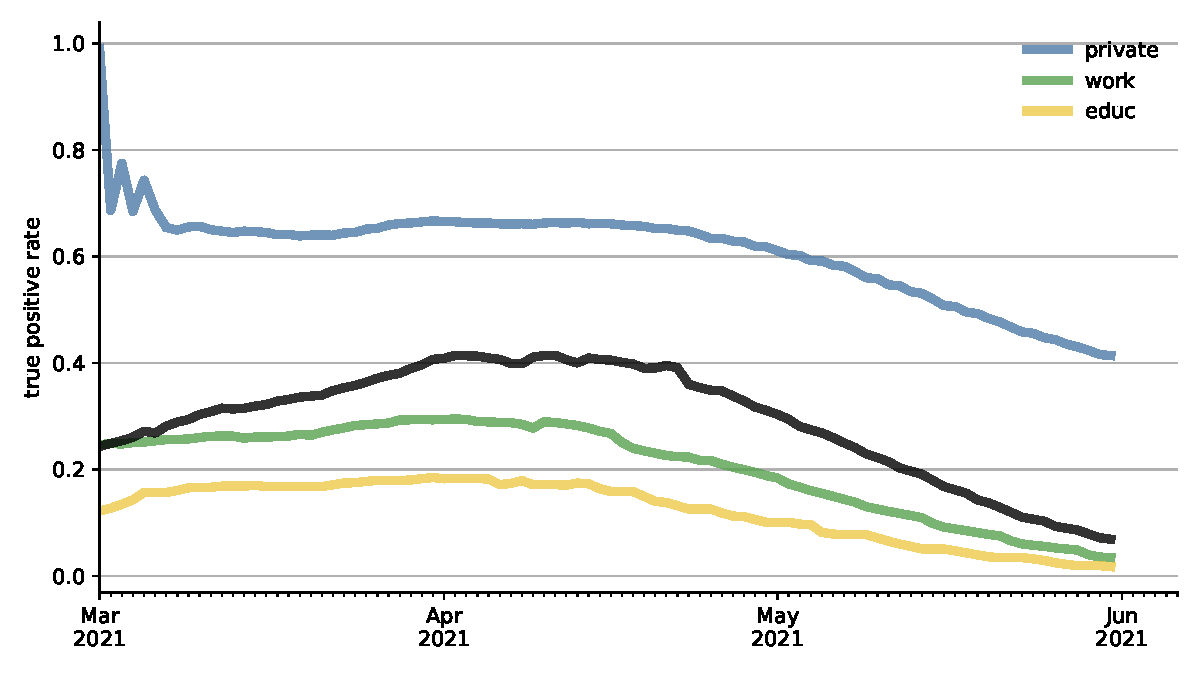
\includegraphics[width=\textwidth]{figures/results/figures/rapid_test_statistics/true_positive_rate}
    %     \caption{Rate of True Positive Rapid Tests by Channel}
    %     \label{fig:rapid_tests_true_positive_rate}
    % \end{subfigure}
    % \hfill
    \begin{subfigure}[b]{0.425\textwidth}
        \centering
        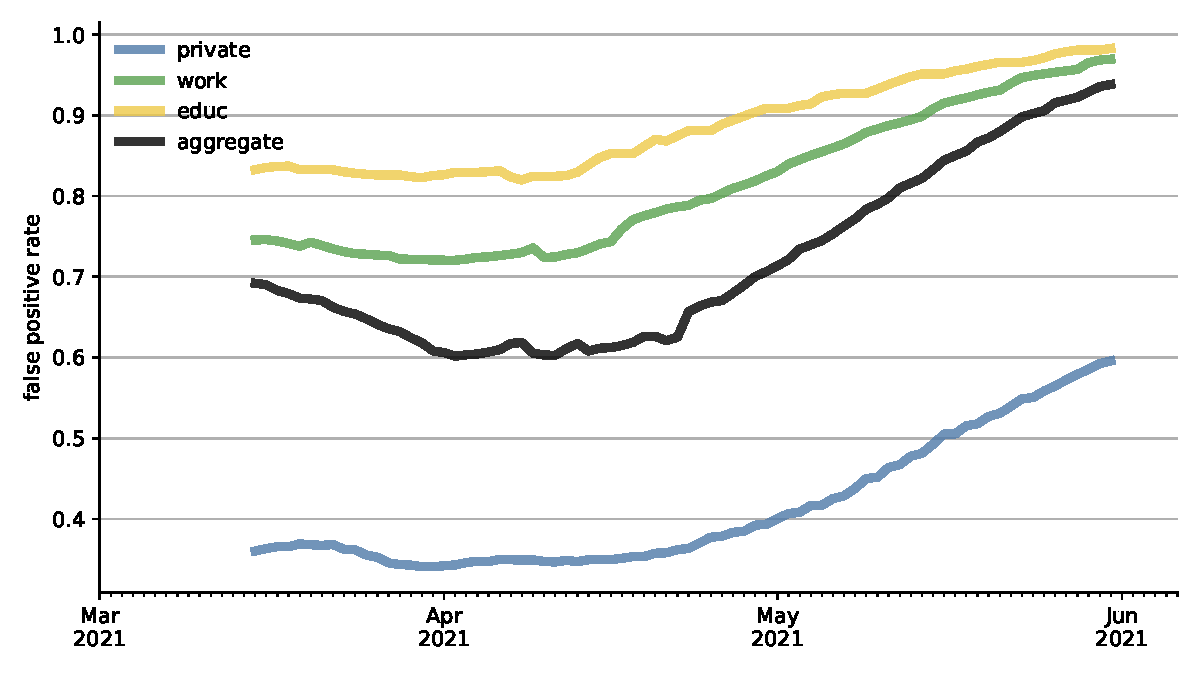
\includegraphics[width=\textwidth]{figures/results/figures/rapid_test_statistics/false_positive_rate}
        \caption{Rate of False Positive Rapid Tests by Channel}
        \label{fig:rapid_tests_false_positive_rate}
    \end{subfigure}
    % \vskip3ex
    % \begin{subfigure}[b]{0.425\textwidth}
    %     \centering
    %     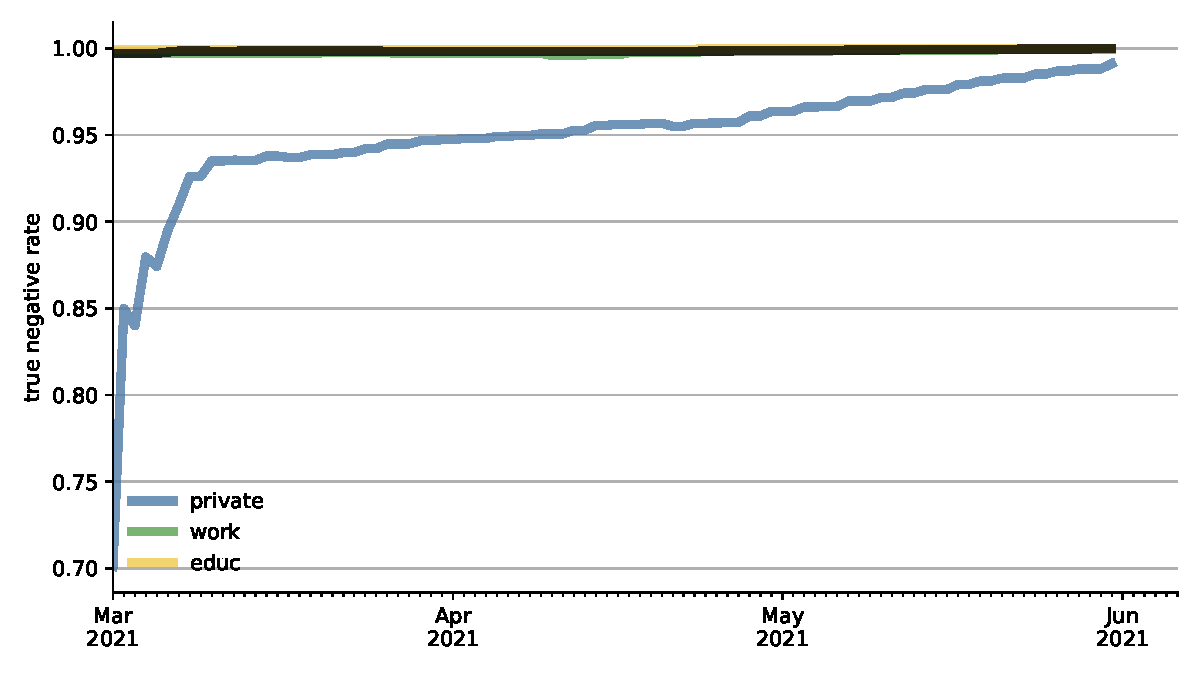
\includegraphics[width=\textwidth]{figures/results/figures/rapid_test_statistics/true_negative_rate}
    %     \caption{Rate of True Negative Rapid Tests by Channel}
    %     \label{fig:rapid_tests_true_negative_rate}
    % \end{subfigure}
    \hfill
    \begin{subfigure}[b]{0.425\textwidth}
        \centering
        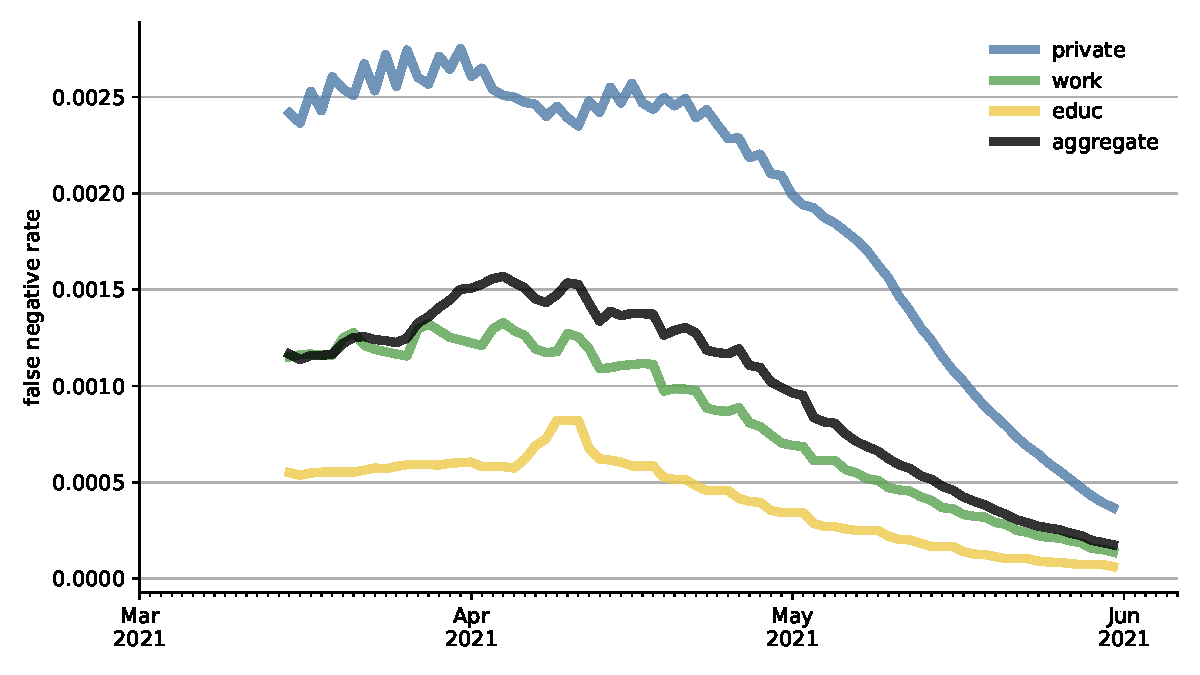
\includegraphics[width=\textwidth]{figures/results/figures/rapid_test_statistics/false_negative_rate}
        \caption{Rate of False Negative Rapid Tests by Channel}
        \label{fig:rapid_tests_false_negative_rate}
    \end{subfigure}
    \vskip3ex
    \caption{Rapid Test Rates by Channel}
    \label{fig:rapid_test_results_rates}

    \floatfoot{\noindent \textit{Note:}
      \textcolor{red}{To be written.}
    }
\end{figure}

\begin{figure} % Share of Tests That Are True Positive / False Positive / True Negative / False Negative
    \centering
    \begin{subfigure}[b]{0.425\textwidth}
        \centering
        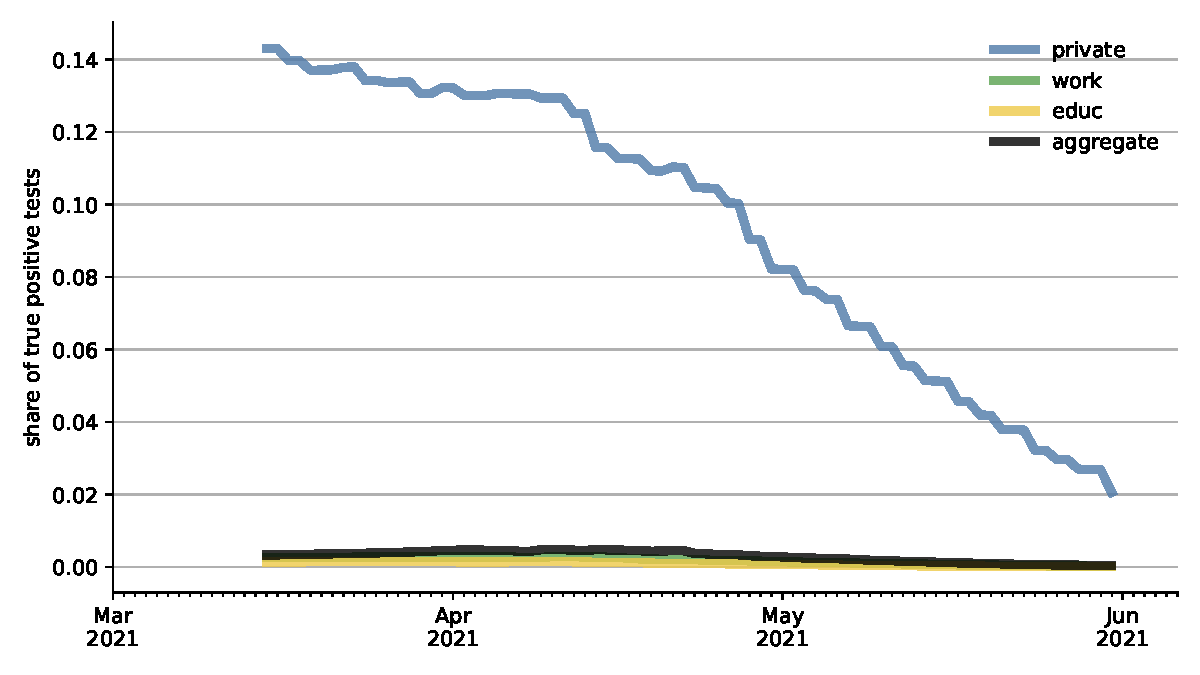
\includegraphics[width=\textwidth]{figures/results/figures/rapid_test_statistics/testshare_true_positive}
        \caption{Share of Tests That Are True Positive by Channel}
        \label{fig:rapid_tests_testshare_true_positive}
    \end{subfigure}
    \hfill
    \begin{subfigure}[b]{0.425\textwidth}
        \centering
        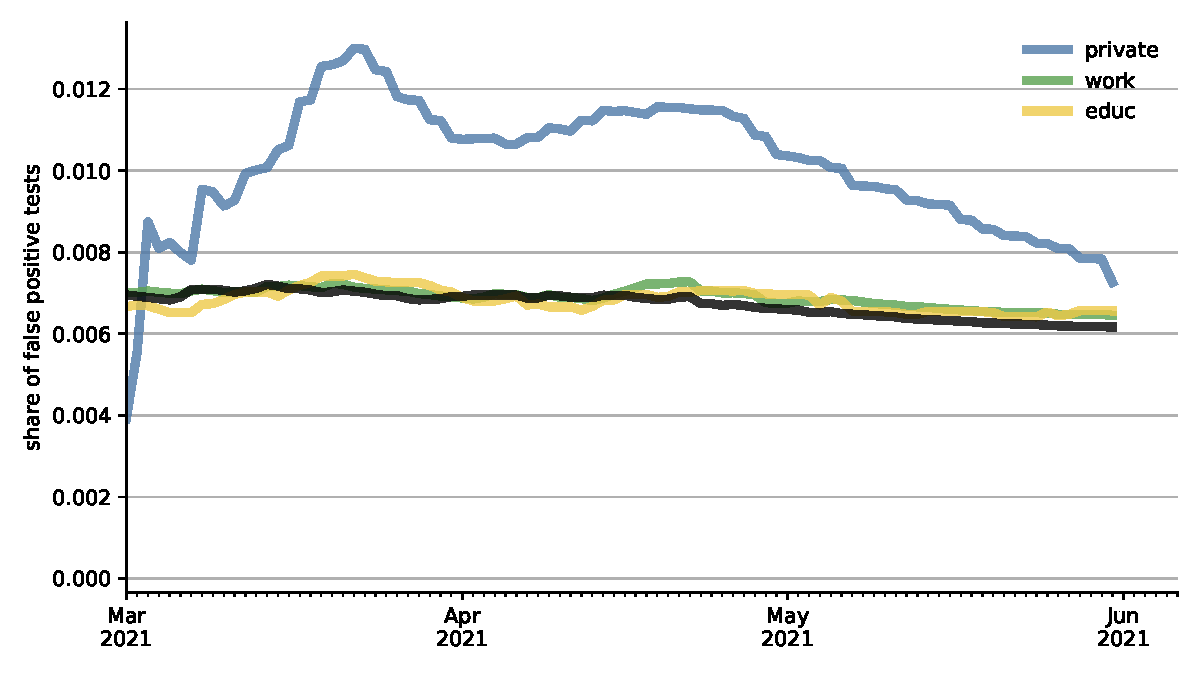
\includegraphics[width=\textwidth]{figures/results/figures/rapid_test_statistics/testshare_false_positive}
        \caption{Share of Tests That Are False Positive by Channel}
        \label{fig:rapid_tests_testshare_false_positive}
    \end{subfigure}
    \vskip3ex
    \begin{subfigure}[b]{0.425\textwidth}
        \centering
        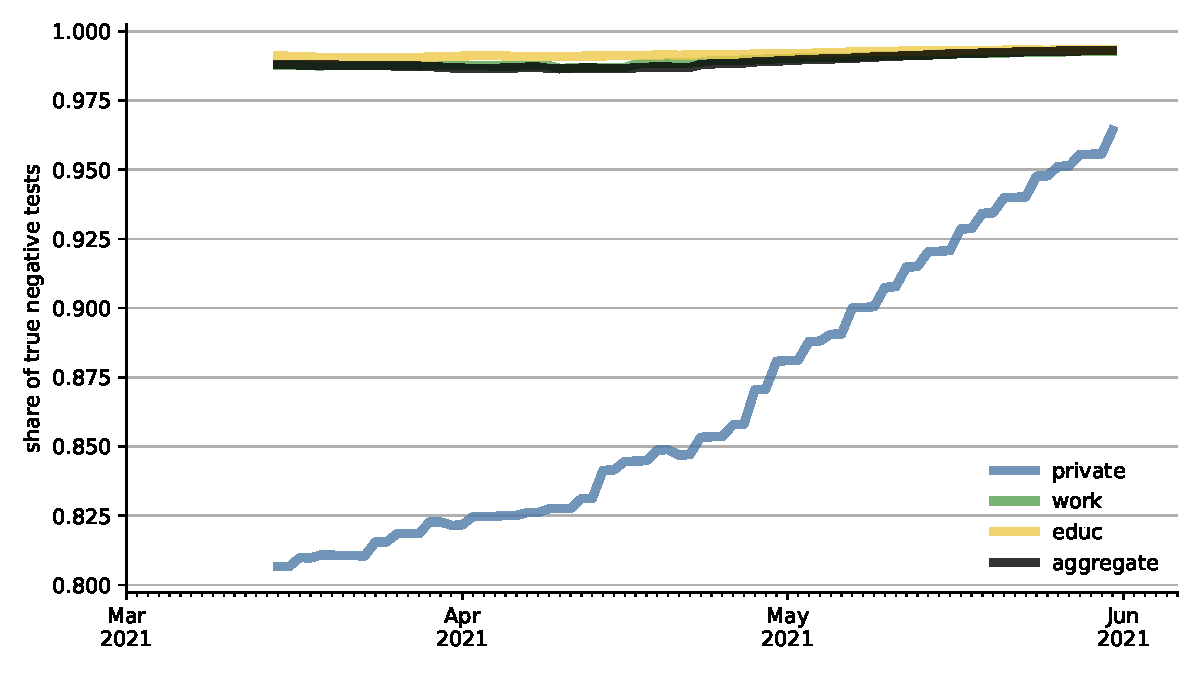
\includegraphics[width=\textwidth]{figures/results/figures/rapid_test_statistics/testshare_true_negative}
        \caption{Share of Tests That Are True Negative by Channel}
        \label{fig:rapid_tests_testshare_true_negative}
    \end{subfigure}
    \hfill
    \begin{subfigure}[b]{0.425\textwidth}
        \centering
        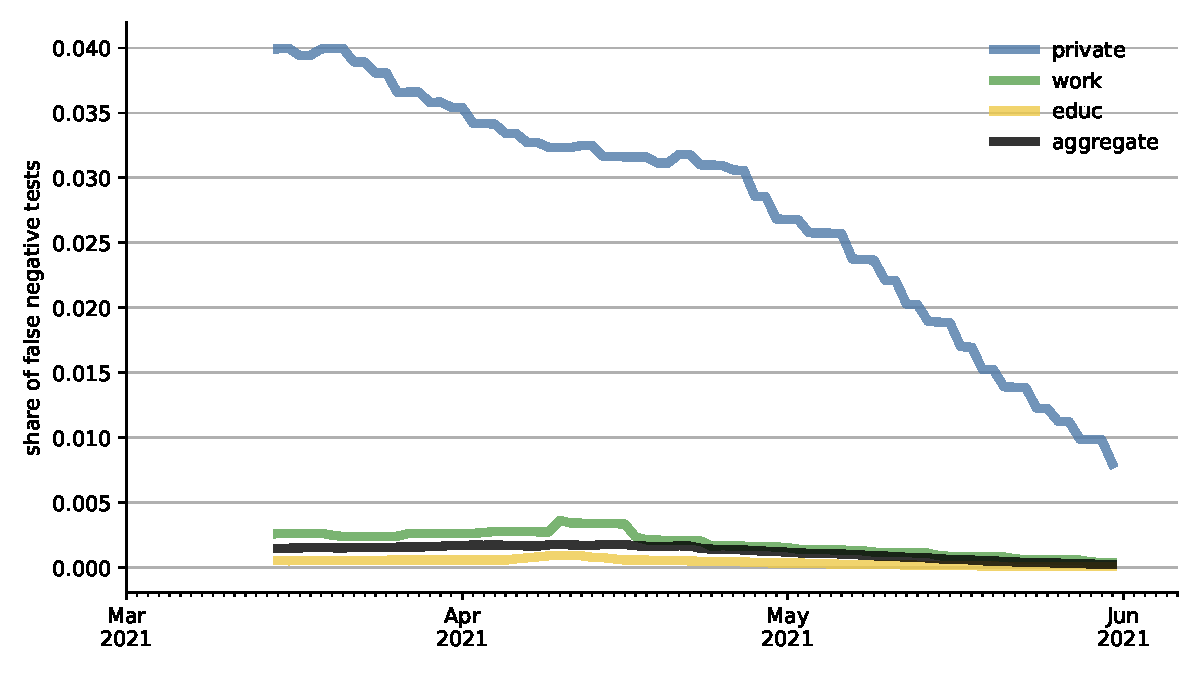
\includegraphics[width=\textwidth]{figures/results/figures/rapid_test_statistics/testshare_false_negative}
        \caption{Share of Tests That Are False Negative by Channel}
        \label{fig:rapid_tests_testshare_false_negative}
    \end{subfigure}
    \vskip3ex
    \caption{Share of Rapid Tests by Outcome and True Infection Status}
    \label{fig:rapid_test_results_test_shares}

    \floatfoot{\noindent \textit{Note:}
      \textcolor{red}{To be written.}
    }
\end{figure}






\FloatBarrier